\setcounter{chapter}{21}
\renewcommand{\thetheorem}{22.a.\arabic{theorem}}
\setcounter{theorem}{0}

\chapter{Euclidean and Hermitian Spaces}

\section{Euclidean and Hermitian (Unitary) Spaces}

At last (!) we endow our spaces with a geometric structure. We work here with vector spaces $V$ over $K = \mathbb{R}$ or $K = \mathbb{C}$. Over $\mathbb{R}$, we will have \qt{Euclidean spaces}. Over $\mathbb{C}$, we will have \qt{Hermitian} (a.k.a.\ unitary) spaces.

% def 22.a.1
\begin{definition}[Scalar Product over $\mathbb{R}$]
\label{def:scalar_product_real}
Let $V$ be a vector space over $\mathbb{R}$. A \qt{scalar product} (a.k.a.\ \qt{inner product}) is a function $V \times V \longrightarrow \mathbb{R}$, denoted by $v, w \mapsto \langle v, w \rangle$ (or $(v,w)$), that has the following properties:
\begin{enumerate}
    \item \textbf{Linearity in the first variable:}
    \begin{align*}
        \langle v_1 + v_2, w \rangle &= \langle v_1, w \rangle + \langle v_2, w \rangle \quad \forall v_1, v_2, w \in V \\
        \langle \alpha v, w \rangle &= \alpha \langle v, w \rangle \quad \forall \alpha \in \mathbb{R}, \; \forall v, w \in V
    \end{align*}
    \item \textbf{Linearity in the second variable:}
    \begin{align*}
        \langle v, w_1 + w_2 \rangle &= \langle v, w_1 \rangle + \langle v, w_2 \rangle \quad \forall v, w_1, w_2 \in V \\
        \langle v, \alpha w \rangle &= \alpha \langle v, w \rangle \quad \forall \alpha \in \mathbb{R}, \; \forall v, w \in V
    \end{align*}
    \item \textbf{Symmetry:}
    \[
        \langle v, w \rangle = \langle w, v \rangle \quad \forall v, w \in V
    \]
    \item \textbf{Positivity:}
    \[
        0 \neq v \in V \implies \langle v, v \rangle > 0
    \]
\end{enumerate}
We call $(V, \langle \cdot, \cdot \rangle)$ a \qt{Euclidean space}, or a space endowed with a scalar product.
\end{definition}

% def 22.a.2
\begin{definition}[Hermitian Product over $\mathbb{C}$]
\label{def:hermitian_product_complex}
Let $V$ be a vector space over $\mathbb{C}$. A \qt{Hermitian product} (or \qt{inner product}) on $V$ is a function $V \times V \longrightarrow \mathbb{C}$, denoted by $v, w \mapsto \langle v, w \rangle$, with the following properties:
\begin{enumerate}
    \item \textbf{Linearity in the first variable:}
    \begin{align*}
        \langle v_1 + v_2, w \rangle &= \langle v_1, w \rangle + \langle v_2, w \rangle \quad \forall v_1, v_2, w \in V \\
        \langle \alpha v, w \rangle &= \alpha \langle v, w \rangle \quad \forall \alpha \in \mathbb{C}, \; \forall v, w \in V
    \end{align*}
    \item \textbf{Sesquilinearity/Conjugate-linearity (complex anti-linearity) in the second variable:}
    \begin{align*}
        \langle v, w_1 + w_2 \rangle &= \langle v, w_1 \rangle + \langle v, w_2 \rangle \quad \forall v, w_1, w_2 \in V \\
        \langle v, \alpha w \rangle &= \overline{\alpha} \langle v, w \rangle \quad \forall \alpha \in \mathbb{C}, \; \forall v, w \in V
    \end{align*}
    \item \textbf{Hermitian property:}
    \[
        \langle v, w \rangle = \overline{\langle w, v \rangle} \quad \forall v, w \in V
    \]
    \item \textbf{Positivity:}
    \[
        0 \neq v \in V \implies \langle v, v \rangle > 0
    \]
\end{enumerate}
We call $(V, \langle \cdot, \cdot \rangle)$ a \qt{Hermitian} (or unitary) space.
\end{definition}

% remark
\begin{remark}[Complex Conjugate and Inner Products]
Recall that if $\alpha = a + ib \in \mathbb{C}$, where $a, b \in \mathbb{R}$ and $i = \sqrt{-1}$, then $\overline{\alpha} := a - ib$ is the complex conjugate of $\alpha$. Recall also, that $\alpha \cdot \overline{\alpha} = a^2 + b^2 = |\alpha|^2 \geq 0$, with equality if and only if $\alpha = 0$.

Note that the definition of a Hermitian product coincides with a scalar product if $V$ is over $\mathbb{R}$, and we allow $\alpha$ only in $\mathbb{R}$.
\end{remark}

% lemma 22.a.3
\begin{lemma}[Basic Properties of the Inner Product]
Let $V$ be a Euclidean or Hermitian vector space. Then:
\begin{enumerate}
    \item $\forall v \in V$, $\langle 0, v \rangle = \langle v, 0 \rangle = 0$.
    \item Let $w \in V$. If $\langle v, w \rangle = 0$ for all $v \in V$, then $w = 0$. (Exercise)
    \item Let $w_1, w_2 \in V$. If $\langle v, w_1 \rangle = \langle v, w_2 \rangle$ for all $v \in V$, then $w_1 = w_2$.
\end{enumerate}
\end{lemma}

% def 22.a.4
\begin{definition}[Norm, Distance, and Orthogonality]
\label{def:norm_distance_orthogonality}
Let $V$ be a Euclidean or Hermitian vector space.
\begin{enumerate}
    \item For all $v \in V$, we define $\|v\| := \sqrt{\langle v, v \rangle} \in \mathbb{R}_{\geq 0}$. The function $\| \cdot \|$ is called the \qt{norm} on $V$ induced by $\langle \cdot, \cdot \rangle$.
    \item A vector $u \in V$ is called a \qt{unit vector} if $\|u\| = 1$. Note that if $0 \neq v \in V$ is any vector, then $\frac{1}{\|v\|}v$ is a unit vector (which is positively proportional to $v$, so it points in the same direction as $v$). We call $\frac{v}{\|v\|}$ the \qt{normalization} of $v$.
    \item For $v, w \in V$, we define the \qt{distance} between $v$ and $w$ by $d(v, w) := \|v - w\|$.
    \item Two vectors $v, w \in V$ are called \qt{orthogonal} (or perpendicular to one another) if $\langle v, w \rangle = 0$. If this is the case, we sometimes write $v \perp w$.
    \item A subset $S \subseteq V$ is called an \qt{orthogonal system} if $0 \notin S$, and for every two distinct elements $v, w \in S$, we have $v \perp w$.
    \item An orthogonal system $S \subseteq V$ is called \qt{orthonormal} if for all $u \in S$, we have $\|u\| = 1$.
\end{enumerate}
\end{definition}

% thm 22.a.5
\begin{theorem}[Pythagoras' Theorem]
\label{thm:pythagoras}
Let $V$ be a Euclidean or Hermitian vector space, and let $v, w \in V$ with $v \perp w$. Then:
\[
    \|v + w\|^2 = \|v\|^2 + \|w\|^2
\]
\end{theorem}

\begin{center}
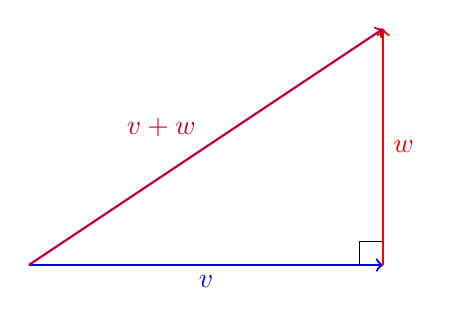
\begin{tikzpicture}[scale=1.5]
    % Define points
    \coordinate (O) at (0,0);
    \coordinate (V) at (3,0);
    \coordinate (VW) at (3,2);
    
    % Draw vectors
    \draw[->, thick, blue] (O) -- (V) node[midway, below] {$v$};
    \draw[->, thick, red] (V) -- (VW) node[midway, right] {$w$};
    \draw[->, thick, purple] (O) -- (VW) node[midway, above left] {$v+w$};
    
    % Right angle symbol
    \draw (2.8, 0) -- (2.8, 0.2) -- (3, 0.2);
\end{tikzpicture}
\end{center}

\begin{proof}
By definition of the norm and the properties of the inner product, we have:
\begin{align*}
    \|v + w\|^2 &= \langle v + w, v + w \rangle \\
    &= \langle v, v \rangle + \langle v, w \rangle + \langle w, v \rangle + \langle w, w \rangle
\end{align*}
Since $v \perp w$, we know that $\langle v, w \rangle = 0$. By Hermitian symmetry, this also implies $\langle w, v \rangle = \overline{\langle v, w \rangle} = \overline{0} = 0$. Therefore, the cross terms vanish, leaving us with:
\begin{align*}
    \|v + w\|^2 &= \|v\|^2 + 0 + 0 + \|w\|^2 \\
    &= \|v\|^2 + \|w\|^2
\end{align*}
\end{proof}

% exercise 1
\begin{exercise}[Generalized Pythagoras' Theorem]
Let $v_1, \dots, v_k \in V$ (where $V$ is a Euclidean or Hermitian space) be mutually orthogonal (i.e., $\langle v_i, v_j \rangle = 0$ for $i \neq j$). Then:
\[
    \|v_1 + \dots + v_k\|^2 = \sum_{i=1}^k \|v_i\|^2
\]
\end{exercise}

% exercise 2
\begin{exercise}[Linear Independence of Orthogonal Systems]
Let $V$ be a Euclidean or Hermitian space. Show that any orthogonal system $S \subseteq V$ is linearly independent.
\end{exercise}

% exercise (page 4)
\begin{exercise}[Reconstructing the Scalar Product from the Norm]
Let $V$ be a Euclidean space. Show that for all $u, v \in V$, we have:
\[
    \langle u, v \rangle = \frac{1}{2}\left(\|u+v\|^2 - \|u\|^2 - \|v\|^2\right) \quad (*)
\]
This shows that the norm $\|\cdot\|$ completely determines the scalar product $\langle\cdot,\cdot\rangle$.
\end{exercise}

% exercise (page 4)
\begin{exercise}[Polarization Identity]
Let $V$ be a Hermitian space. Then:
\[
    \langle u, v \rangle = \frac{1}{4}\left(\|u+v\|^2 - \|u-v\|^2 + i\|u+iv\|^2 - i\|u-iv\|^2\right) \quad (**)
\]
\end{exercise}

\begin{importantremark}[The Parallelogram Law]
\label{rem:parallelogram_law}
Warning: For general norms $\|\cdot\|$, one cannot necessarily find a scalar product that induces it. A norm $\|\cdot\|$ comes from a scalar product if and only if it satisfies the \qt{Parallelogram law}:
\[
    \|u+v\|^2 + \|u-v\|^2 = 2\left(\|u\|^2 + \|v\|^2\right)
\]
\end{importantremark}

\subsection{Examples}

% examples (page 5)
\begin{example}[Standard and Matrix-Induced Inner Products]
\leavevmode
\begin{enumerate}
    \item Standard inner products on $\mathbb{R}^n$ and $\mathbb{C}^n$:
    \begin{align*}
        \langle x, y \rangle_{\mathbb{R}^n} &= \sum_{i=1}^n x_i y_i \\
        \langle z, w \rangle_{\mathbb{C}^n} &= \sum_{i=1}^n z_i \overline{w}_i
    \end{align*}
    
    \item Let $A \in \M_{n \times n}(\mathbb{R})$ be a symmetric matrix. Define a function $V \times V \longrightarrow \mathbb{R}$ by:
    \[
        \langle v, w \rangle_A = v^T A w
    \]
    Check that properties (1)--(3) of a scalar product hold for \textit{any} symmetric matrix $A$. Specifically, for symmetry, we have:
    \[
        \langle w, v \rangle_A = w^T A v = (w^T A v)^T = v^T A^T w = v^T A w = \langle v, w \rangle_A
    \]
    (Note that $w^T A v$ is a $1 \times 1$ matrix, and is therefore equal to its transpose).
    
    What about property (4), positivity? For example, let $A = \begin{pmatrix} 1 & 0 \\ 0 & -1 \end{pmatrix}$, which is symmetric. Then:
    \[
        \left\langle \begin{pmatrix} x_1 \\ x_2 \end{pmatrix}, \begin{pmatrix} y_1 \\ y_2 \end{pmatrix} \right\rangle_A = x_1 y_1 - x_2 y_2
    \]
    But taking $v = \begin{pmatrix} 0 \\ 1 \end{pmatrix}$, we get:
    \[
        \left\langle \begin{pmatrix} 0 \\ 1 \end{pmatrix}, \begin{pmatrix} 0 \\ 1 \end{pmatrix} \right\rangle_A = -1 < 0
    \]
    So, there is a lack of positivity.
\end{enumerate}
\end{example}




\subsection{Matrices and Positive Definiteness}

% Def. (22.a.6)
\begin{definition}[Symmetric Matrix]
    A matrix $A \in \M_{n \times n}(K)$ (where $K$ is any field) is called \qt{symmetric} if $A^T = A$ (i.e., $a_{ij} = a_{ji}$ for all $i,j$).
\end{definition}

% Def. (22.a.7)
\begin{definition}[Adjoint and Hermitian Matrices]
    \begin{enumerate}
        \item Let $A \in \M_{n \times m}(\mathbb{C})$. We write $\overline{A}$ for the matrix whose entry at index $(i,j)$ is $\overline{A_{ij}}$, representing complex conjugation. Thus, $(\overline{A})_{ij} := \overline{A_{ij}}$.
        \item Let $A \in \M_{n \times m}(\mathbb{C})$. We define $A^* := \overline{A}^T \in \M_{m \times n}(\mathbb{C})$. The matrix $A^*$ is called the \qt{adjoint matrix} of $A$ (this has nothing to do with the classical adjoint, $\operatorname{adj}(A)$).
        \item A matrix $A \in \M_{n \times n}(\mathbb{C})$ is called \qt{Hermitian} if $A^* = A$ (which is equivalent to $A = \overline{A}^T$).
    \end{enumerate}
\end{definition}

\begin{example}[Important example]
    Let $A \in \M_{n \times n}(\mathbb{R})$. Define $\langle \cdot, \cdot \rangle_A : \mathbb{R}^n \times \mathbb{R}^n \to \mathbb{R}$ by
    \begin{equation*}
        \langle v, w \rangle_A = v^T \cdot A \cdot w.
    \end{equation*}
    
    \begin{exercise}
        Show that $\langle \cdot, \cdot \rangle_A$ is bilinear (i.e., linear in both variables).
    \end{exercise}
    
    Assume now that $A$ is symmetric. Then, $\langle v, w \rangle_A = \langle w, v \rangle_A$ for all $v, w$. Indeed,
    \begin{equation*}
        \langle w, v \rangle_A = w^T \cdot A \cdot v = w^T A^T v = (v^T A w)^T = (\langle v, w \rangle_A)^T = \langle v, w \rangle_A.
    \end{equation*}
    (Note that $v^T A w$ is just a scalar, which can be viewed as a $1 \times 1$ matrix, hence it equals its own transpose). 
    
    Is $\langle \cdot, \cdot \rangle_A$ a scalar product? In general, it is not. For example, consider $A = \left(\begin{smallmatrix} -1 & 0 \\ 0 & -1 \end{smallmatrix}\right)$. Then, $\langle \left(\begin{smallmatrix} 0 \\ 1 \end{smallmatrix}\right), \left(\begin{smallmatrix} 0 \\ 1 \end{smallmatrix}\right) \rangle_A = -1$. However, for a scalar product, we need $\langle v, v \rangle > 0$ for all $v \neq 0$. Therefore, we lack positivity here.
\end{example}

% Def. (22.a.8)
\begin{definition}[Positive Definite Matrix (Real Case)]
    A symmetric matrix $A \in \M_{n \times n}(\mathbb{R})$ is called \qt{positive definite} if $v^T A v > 0$ for all $0 \neq v \in \mathbb{R}^n$.
\end{definition}

\begin{claim*}
    If $A$ is positive definite, then $\langle \cdot, \cdot \rangle_A$ is a scalar product.
\end{claim*}

\begin{example}
    \begin{enumerate}
        \item Let $a_1, \dots, a_n > 0$ (with $a_i \in \mathbb{R}$). Then, the diagonal matrix
        \begin{equation*}
            D = \begin{pmatrix} a_1 & & 0 \\ & \ddots & \\ 0 & & a_n \end{pmatrix}
        \end{equation*}
        is positive definite. Indeed, if $v = \begin{pmatrix} v_1 \\ \vdots \\ v_n \end{pmatrix}$, then
        \begin{equation*}
            \langle v, v \rangle_D = v^T \cdot D \cdot v = a_1 v_1^2 + \dots + a_n v_n^2 \geq 0,
        \end{equation*}
        with equality if and only if $v_i = 0$ for all $i$.
        \item Let $A = \begin{pmatrix} a & b \\ b & d \end{pmatrix} \in \M_{2 \times 2}(\mathbb{R})$. Then, $A$ is positive definite if and only if $a > 0$ and $\det(A) > 0$ (Exercise).
    \end{enumerate}
\end{example}

The situation for Hermitian products is similar.

% Def. (22.a.9)
\begin{definition}[Positive Definite Matrix (Complex Case)]
    Let $A \in \M_{n \times n}(\mathbb{C})$ be a Hermitian matrix. We say that $A$ is \qt{positive definite} if for all $0 \neq v \in \mathbb{C}^n$, we have $v^T A \overline{v} > 0$. 
\end{definition}

\begin{remark}
    Note that $v^T A \overline{v} \in \mathbb{R}$, because
    \begin{equation*}
        \overline{(v^T A \overline{v})} = \overline{v}^T \overline{A} v = (\overline{v}^T \overline{A} v)^T = v^T \overline{A}^T \overline{v} = v^T A \overline{v}.
    \end{equation*}
    Here, we used the facts that for a $1 \times 1$ matrix (a scalar), $(\cdot)^T = (\cdot)$, and that $A$ is Hermitian (so $\overline{A}^T = A$). Also, recall that if $v = \begin{pmatrix} v_1 \\ \vdots \\ v_n \end{pmatrix} \in \mathbb{C}^n$, then $\overline{v} := \begin{pmatrix} \overline{v}_1 \\ \vdots \\ \overline{v}_n \end{pmatrix}$.
\end{remark}

Given a positive definite complex matrix $A$, we can define a Hermitian product on $\mathbb{C}^n$ by
\begin{equation*}
    \langle v, w \rangle_A = v^T A \overline{w}.
\end{equation*}

\begin{claim*}
    The operation $\langle \cdot, \cdot \rangle_A$ is a Hermitian product if and only if $A$ is positive definite.
\end{claim*}

\begin{exercise}
    A matrix $A = \begin{pmatrix} a & b \\ \overline{b} & d \end{pmatrix} \in \M_{2 \times 2}(\mathbb{C})$ is positive definite if and only if $a > 0$, $\det A \in \mathbb{R}$, and $\det A > 0$.
\end{exercise}

\begin{proof}[Proof of the Claim]
    We will prove it for complex matrices and Hermitian products (the case of symmetric matrices and scalar products is very similar and even simpler, which is left as an exercise). 
    
    Let $A \in \M_{n \times n}(\mathbb{C})$ and suppose that $\langle v, w \rangle_A := v^T A \overline{w}$ is a Hermitian product. For all $v, w$, we have 
    \begin{equation}\langle v, w \rangle_A = \overline{\langle w, v \rangle}_A,\end{equation} 
    which implies
    \begin{equation*}
        v^T A \overline{w} = \overline{w^T A \overline{v}}.
    \end{equation*}
    This simplifies as follows:
    \begin{equation*}
        v^T A \overline{w} = \overline{w}^T \overline{A} v \implies v^T A \overline{w} = (\overline{w}^T \overline{A} v)^T \implies v^T A \overline{w} = v^T \overline{A}^T \overline{w}.
    \end{equation*}
    Take $v = e_i$ and $w = e_j$ (the standard basis vectors). Write $A$ as
    \begin{equation*}
        A = \begin{pmatrix} a_{11} & \dots & a_{1j} & \dots & a_{1n} \\ \vdots & & \vdots & & \vdots \\ a_{n1} & \dots & a_{nj} & \dots & a_{nn} \end{pmatrix}.
    \end{equation*}
    Then,
    \begin{equation*}
        e_i^T \cdot A \cdot e_j = \begin{pmatrix} 0 & \dots & 1 & \dots & 0 \end{pmatrix} A \begin{pmatrix} 0 \\ \vdots \\ 1 \\ \vdots \\ 0 \end{pmatrix} = \begin{pmatrix} 0 & \dots & 1 & \dots & 0 \end{pmatrix} \begin{pmatrix} a_{1j} \\ \vdots \\ a_{nj} \end{pmatrix} = a_{ij}.
    \end{equation*}
    Similarly, $e_i^T \overline{A}^T e_j = \overline{a}_{ji}$. Therefore, $a_{ij} = \overline{a}_{ji}$ for all $i, j$, which means $\overline{A}^T = A$, proving that $A$ is Hermitian. 
    
    The fact that $A$ is positive definite is precisely the condition that $\langle v, v \rangle_A > 0$ for all $v \neq 0$, which translates to $v^T A \overline{v} > 0$.
    
    The opposite statement, that if $A$ is positive definite then $\langle \cdot, \cdot \rangle_A$ is a Hermitian product, is left as an exercise.
\end{proof}

\subsection{The geometry on $V$ and the choice of inner product}

The geometry on $V$ depends on the choice of inner product.

\begin{example}
    Let $V = \mathbb{R}^2$. Let $\langle v, w \rangle = v_1 w_1 + v_2 w_2$ be the standard scalar product on $\mathbb{R}^2$. 
    We define another product $\langle v, w \rangle' = a_1 v_1 w_1 + a_2 v_2 w_2$, where $a_1, a_2 > 0$. 
    Notice that this is exactly $\langle v, w \rangle_A$ for the matrix $A = \begin{pmatrix} a_1 & 0 \\ 0 & a_2 \end{pmatrix}$.
    
    The unit sphere for the standard product $\langle \cdot, \cdot \rangle$ is:
    \begin{equation*}
        S = \{v \in \mathbb{R}^2 \mid \|v\| = 1\} = \{(v_1, v_2) \mid v_1^2 + v_2^2 = 1\}.
    \end{equation*}
    The unit sphere for $\langle \cdot, \cdot \rangle'$ is:
    \begin{equation*}
        S' = \{v \in \mathbb{R}^2 \mid \|v\|' = 1\} = \{(v_1, v_2) \mid a_1 v_1^2 + a_2 v_2^2 = 1\}.
    \end{equation*}

    \begin{center}
        \begin{minipage}{0.45\textwidth}
            \centering
            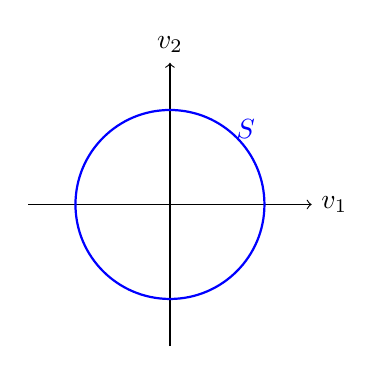
\begin{tikzpicture}[scale=1.2]
                \draw[->] (-1.5,0) -- (1.5,0) node[right] {$v_1$};
                \draw[->] (0,-1.5) -- (0,1.5) node[above] {$v_2$};
                \draw[thick, blue] (0,0) circle (1);
                \node[blue] at (0.8, 0.8) {$S$};
            \end{tikzpicture}
        \end{minipage}
        \begin{minipage}{0.45\textwidth}
            \centering
            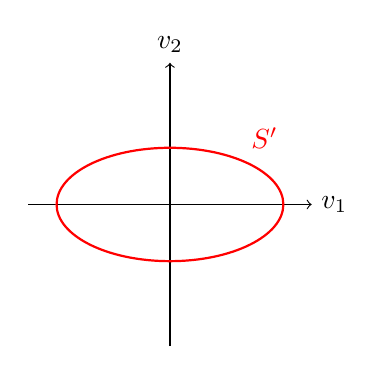
\begin{tikzpicture}[scale=1.2]
                \draw[->] (-1.5,0) -- (1.5,0) node[right] {$v_1$};
                \draw[->] (0,-1.5) -- (0,1.5) node[above] {$v_2$};
                \draw[thick, red] (0,0) ellipse (1.2 and 0.6);
                \node[red] at (1.0, 0.7) {$S'$};
            \end{tikzpicture}
        \end{minipage}
    \end{center}
\end{example}

\begin{example}
    Let $A = \begin{pmatrix} 1 & -1 \\ -1 & 2 \end{pmatrix}$. This matrix is positive definite (why?). 
    Let $\langle \cdot, \cdot \rangle$ be the standard scalar product, and define $\langle \cdot, \cdot \rangle' := \langle \cdot, \cdot \rangle_A$.
    
    We compute:
    \begin{equation*}
        \left\langle \begin{pmatrix} 1 \\ 0 \end{pmatrix}, \begin{pmatrix} 1 \\ 1 \end{pmatrix} \right\rangle = 1.
    \end{equation*}
    However, using the modified product:
    \begin{equation*}
        \left\langle \begin{pmatrix} 1 \\ 0 \end{pmatrix}, \begin{pmatrix} 1 \\ 1 \end{pmatrix} \right\rangle' = \begin{pmatrix} 1 & 0 \end{pmatrix} \begin{pmatrix} 1 & -1 \\ -1 & 2 \end{pmatrix} \begin{pmatrix} 1 \\ 1 \end{pmatrix} = \begin{pmatrix} 1 & -1 \end{pmatrix} \begin{pmatrix} 1 \\ 1 \end{pmatrix} = 0.
    \end{equation*}
    So, $\left(\begin{smallmatrix} 1 \\ 0 \end{smallmatrix}\right) \perp' \left(\begin{smallmatrix} 1 \\ 1 \end{smallmatrix}\right)$, but $\left(\begin{smallmatrix} 1 \\ 0 \end{smallmatrix}\right) \not\perp \left(\begin{smallmatrix} 1 \\ 1 \end{smallmatrix}\right)$.

    \begin{center}
        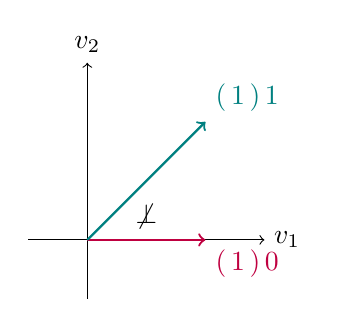
\begin{tikzpicture}[scale=1.5]
            \draw[->] (-0.5,0) -- (1.5,0) node[right] {$v_1$};
            \draw[->] (0,-0.5) -- (0,1.5) node[above] {$v_2$};
            \draw[->, thick, purple] (0,0) -- (1,0) node[below right] {$\begin{pmatrix} 1 \\ 0 \end{pmatrix}$};
            \draw[->, thick, teal] (0,0) -- (1,1) node[above right] {$\begin{pmatrix} 1 \\ 1 \end{pmatrix}$};
            \node at (0.5, 0.2) {$\not\perp$};
        \end{tikzpicture}
    \end{center}
\end{example}

\subsection{A different type of example}

\begin{example}[A different type of example]
    Let $C[a,b]$ be the space of continuous functions $f: [a,b] \to \mathbb{R}$. It is a vector space over $\mathbb{R}$ with respect to the standard operations. 
    We define a scalar product:
    \begin{equation*}
        \langle f, g \rangle := \int_a^b f(x) \cdot g(x) \, dx.
    \end{equation*}
    This is well-defined and finite. (Why?)
\end{example}

\begin{exercise}
    Show that $\langle \cdot, \cdot \rangle$ is linear in both variables and symmetric.
\end{exercise}

Let us check positivity: let $0 \neq f \in C[a,b]$.
\begin{equation*}
    \langle f, f \rangle = \int_a^b (f(x))^2 \, dx.
\end{equation*}
Since $f \neq 0$, there exists an $x_0 \in (a,b)$ such that $f(x_0) \neq 0$. Since $f$ is continuous, so is $f^2$. Hence, there exists a $\delta > 0$ such that $[x_0 - \delta, x_0 + \delta] \subseteq [a,b]$ and $f(x) \neq 0$ for all $x \in [x_0 - \delta, x_0 + \delta]$. This implies that $(f(x))^2 > 0$ for all $x \in [x_0 - \delta, x_0 + \delta]$. Therefore,

\begin{equation*}
    \langle f, f \rangle = \int_a^b (f(x))^2 \, dx \geq \int_{x_0 - \delta}^{x_0 + \delta} (f(x))^2 \, dx \geq 2\delta \cdot \min_{x \in [x_0-\delta, x_0+\delta]} (f(x))^2 > 0.
\end{equation*}

\begin{remark}
    By this scalar product on $C[-\pi, \pi]$, the functions $f(x) = \sin x$ and $g(x) \equiv 1$ are orthogonal.
\end{remark}

\subsection{Norms and Angles}

% Def. (22.a.10)
\begin{definition}[Norm]
    Let $V$ be a vector space over $K$ (where $K = \mathbb{R}$ or $\mathbb{C}$). A \qt{norm} on $V$ is a function $\| \cdot \|: V \to \mathbb{R}_{\geq 0}$ such that:
    \begin{enumerate}
        \item $\|u + v\| \leq \|u\| + \|v\|$ for all $u, v \in V$ (Triangle inequality).
        \item $\|\alpha \cdot v\| = |\alpha| \cdot \|v\|$ for all $\alpha \in K$ and $v \in V$ (Homogeneity).
        \item If $\|v\| = 0$, then $v = 0$ (Non-degeneracy).
    \end{enumerate}
\end{definition}

\begin{claim*}
    If $\langle \cdot, \cdot \rangle$ is an inner product on $V$, then $\|v\| := \sqrt{\langle v, v \rangle}$ is a norm on $V$. We will prove this soon.
\end{claim*}

\begin{exercise}
    For $\left(\begin{smallmatrix} a \\ b \end{smallmatrix}\right) \in \mathbb{R}^2$, define $\left\| \left(\begin{smallmatrix} a \\ b \end{smallmatrix}\right) \right\|' := \max\{|a|, |b|\}$, and $\left\| \left(\begin{smallmatrix} a \\ b \end{smallmatrix}\right) \right\|'' := |a| + |b|$. 
    Show that $\| \cdot \|'$ and $\| \cdot \|''$ are norms, but they are not induced by any scalar product. 
    
    \textit{Hint:} Recall that if the scalar product $\langle \cdot, \cdot \rangle$ induces $\| \cdot \|$, then $\langle u, w \rangle = \frac{1}{2} (\|u + w\|^2 - \|u\|^2 - \|w\|^2)$.
\end{exercise}

% Thm. (22.a.11)
\begin{theorem}[Cauchy-Schwarz Inequality]
    \label{thm:cauchy_schwarz}
    Let $V$ be a Euclidean or Hermitian space. For all $u, v \in V$, we have
    \begin{equation*}
        |\langle u, v \rangle| \leq \|u\| \cdot \|v\|.
    \end{equation*}
    Furthermore, equality holds if and only if $u$ and $v$ are linearly dependent.
\end{theorem}

\begin{proof}
    If $v = 0$, then both sides are $0$, and the inequality holds (with equality). Since $v = 0$, the vectors $u$ and $v$ are linearly dependent, and therefore, the second statement also holds.
    
    Assume now that $v \neq 0$. For any scalar $\lambda \in K$ (where $K = \mathbb{R}$ or $\mathbb{C}$), we have, by the positivity of the inner product,
    \begin{equation*}
        0 \leq \langle u - \lambda v, u - \lambda v \rangle.
    \end{equation*}
    Using the linearity in the first variable and conjugate-linearity (or linearity) in the second variable, we expand this to obtain
    \begin{equation*}
        0 \leq \langle u, u \rangle - \lambda \langle v, u \rangle - \overline{\lambda} \langle u, v \rangle + \lambda \overline{\lambda} \langle v, v \rangle.
    \end{equation*}
    Choose $\lambda = \frac{\langle u, v \rangle}{\|v\|^2}$. Substituting this into the inequality yields
    \begin{align*}
        0 &\leq \|u\|^2 - \frac{\langle u, v \rangle}{\|v\|^2} \langle v, u \rangle - \frac{\overline{\langle u, v \rangle}}{\|v\|^2} \langle u, v \rangle + \frac{\langle u, v \rangle \overline{\langle u, v \rangle}}{\|v\|^4} \|v\|^2 \\
        &= \|u\|^2 - \frac{\langle u, v \rangle \overline{\langle u, v \rangle}}{\|v\|^2} - \frac{\overline{\langle u, v \rangle} \langle u, v \rangle}{\|v\|^2} + \frac{\langle u, v \rangle \overline{\langle u, v \rangle}}{\|v\|^2} \\
        &= \|u\|^2 - \frac{|\langle u, v \rangle|^2}{\|v\|^2}.
    \end{align*}
    Multiplying by $\|v\|^2$ (which is strictly positive), we obtain
    \begin{equation*}
        0 \leq \|u\|^2 \|v\|^2 - |\langle u, v \rangle|^2 \implies |\langle u, v \rangle|^2 \leq \|u\|^2 \|v\|^2.
    \end{equation*}
    Taking the square root of both sides gives the Cauchy-Schwarz inequality.
    
    For the equality condition, notice that equality holds if and only if $\langle u - \lambda v, u - \lambda v \rangle = 0$. By the non-degeneracy of the inner product, this is equivalent to $u - \lambda v = 0$, meaning $u = \lambda v$. Therefore, equality holds if and only if $u$ and $v$ are linearly dependent.
\end{proof}

% Cor. (22.a.12)
\begin{corollary}
    If $\langle \cdot, \cdot \rangle$ is an inner product on $V$, then $\|v\| := \sqrt{\langle v, v \rangle}$ is a norm on $V$.
\end{corollary}

\begin{proof}
    The positivity and homogeneity properties are straightforward to verify. We will show the triangle inequality, namely $\|u + v\| \leq \|u\| + \|v\|$. We compute
    \begin{align*}
        \|u + v\|^2 &= \langle u + v, u + v \rangle \\
        &= \langle u, u \rangle + \langle u, v \rangle + \langle v, u \rangle + \langle v, v \rangle \\
        &= \|u\|^2 + \langle u, v \rangle + \overline{\langle u, v \rangle} + \|v\|^2 \\
        &= \|u\|^2 + 2 \operatorname{Re}(\langle u, v \rangle) + \|v\|^2.
    \end{align*}
    Since $\operatorname{Re}(z) \leq |z|$ for any complex number $z$, and applying the Cauchy-Schwarz inequality, we get
    \begin{equation*}
        \|u + v\|^2 \leq \|u\|^2 + 2 |\langle u, v \rangle| + \|v\|^2 \leq \|u\|^2 + 2 \|u\| \|v\| + \|v\|^2 = (\|u\| + \|v\|)^2.
    \end{equation*}
    Taking the square root yields the desired result.
\end{proof}

% Def. (22.a.13)
\begin{definition}[Angle]
    Let $V$ be a Euclidean space. For any two non-zero vectors $u, v \in V$, we define the \qt{angle} $\alpha$ between them by the equation
    \begin{equation*}
        \cos \alpha = \frac{\langle u, v \rangle}{\|u\| \cdot \|v\|},
    \end{equation*}
    where $\alpha \in [0, \pi]$. The Cauchy-Schwarz inequality guarantees that $-1 \leq \frac{\langle u, v \rangle}{\|u\| \cdot \|v\|} \leq 1$, so this definition is well-posed.
\end{definition}

\begin{definition*}[Orthogonality]
    Let $V$ be a Euclidean or Hermitian space. We say that $u, v \in V$ are \qt{orthogonal} if $\langle u, v \rangle = 0$. In this case, we write $u \perp v$.
\end{definition*}

\begin{example}
    In $\mathbb{R}^2$ with the standard scalar product, the vectors $e_1 = \left(\begin{smallmatrix} 1 \\ 0 \end{smallmatrix}\right)$ and $e_2 = \left(\begin{smallmatrix} 0 \\ 1 \end{smallmatrix}\right)$ are orthogonal.
\end{example}

\begin{remark}
    The relationship between orthogonality and the norm is captured by the Pythagorean Theorem (Theorem \ref{thm:pythagoras}), which states that for orthogonal vectors $u$ and $v$, the squared norm of their sum is the sum of their squared norms: $\|u+v\|^2 = \|u\|^2 + \|v\|^2$.
\end{remark}


\subsection{The Gram-Schmidt Orthogonalization Process}

% Thm. (22.a.14)
\begin{theorem}[Properties of Orthogonal Systems]
    Let $V$ be a Euclidean or Hermitian space, and let $(v_1, \dots, v_k)$ be an orthogonal system of non-zero vectors in $V$. Then:
    \begin{itemize}
        \item The vectors $v_1, \dots, v_k$ are linearly independent.
        \item If $v \in \Sp(v_1, \dots, v_k)$, meaning $v = \sum_{i=1}^k \alpha_i v_i$, then the coefficients are given by
        \begin{equation*}
            \alpha_i = \frac{\langle v, v_i \rangle}{\|v_i\|^2} \quad \text{for all } 1 \leq i \leq k.
        \end{equation*}
    \end{itemize}
\end{theorem}

\begin{proof}
    We prove the second property first. Suppose $v = \sum_{j=1}^k \alpha_j v_j$. Taking the inner product with $v_i$ yields
    \begin{equation*}
        \langle v, v_i \rangle = \left\langle \sum_{j=1}^k \alpha_j v_j, v_i \right\rangle = \sum_{j=1}^k \alpha_j \langle v_j, v_i \rangle.
    \end{equation*}
    Since the system is orthogonal, $\langle v_j, v_i \rangle = 0$ for all $j \neq i$. Thus, the sum collapses to a single term:
    \begin{equation*}
        \langle v, v_i \rangle = \alpha_i \langle v_i, v_i \rangle = \alpha_i \|v_i\|^2.
    \end{equation*}
    Since $v_i \neq 0$, we have $\|v_i\|^2 > 0$. Dividing by $\|v_i\|^2$, we obtain
    \begin{equation*}
        \alpha_i = \frac{\langle v, v_i \rangle}{\|v_i\|^2}.
    \end{equation*}
    
    To prove the first property, assume that there exist scalars $\alpha_1, \dots, \alpha_k \in K$ such that $\sum_{i=1}^k \alpha_i v_i = 0$. By the formula we just established, the coefficients are given by
    \begin{equation*}
        \alpha_i = \frac{\langle 0, v_i \rangle}{\|v_i\|^2} = 0.
    \end{equation*}
    Since $\alpha_i = 0$ for all $1 \leq i \leq k$, the vectors $v_1, \dots, v_k$ are linearly independent.
\end{proof}

% Prop. (22.a.15)
\begin{proposition}[Matrix Representation in Orthonormal Bases]
    Let $V$ and $W$ be Euclidean or Hermitian spaces. Let $\mathcal{B} = (v_1, \dots, v_n)$ be an orthonormal basis of $V$, and let $\mathcal{C} = (w_1, \dots, w_m)$ be an orthonormal basis of $W$. Let $T: V \to W$ be a linear transformation. Then the entries of the representation matrix $A = [T]_{\mathcal{C}}^{\mathcal{B}} \in \M_{m \times n}(K)$ are given by:
    \begin{equation*}
        A_{ij} = \langle T(v_j), w_i \rangle,
    \end{equation*}
    for $1 \leq i \leq m$ and $1 \leq j \leq n$.
\end{proposition}

\begin{proof}
    By definition of the representation matrix $[T]_{\mathcal{C}}^{\mathcal{B}}$, the $j$-th column of $A$ consists of the coordinates of $T(v_j)$ with respect to the basis $\mathcal{C}$. That is,
    \begin{equation*}
        T(v_j) = \sum_{i=1}^m A_{ij} w_i.
    \end{equation*}
    Taking the inner product of both sides with $w_k$ (for some $1 \leq k \leq m$), we obtain
    \begin{equation*}
        \langle T(v_j), w_k \rangle = \left\langle \sum_{i=1}^m A_{ij} w_i, w_k \right\rangle = \sum_{i=1}^m A_{ij} \langle w_i, w_k \rangle.
    \end{equation*}
    Since $\mathcal{C}$ is an orthonormal basis, $\langle w_i, w_k \rangle = \delta_{ik}$ (which is $1$ if $i=k$ and $0$ otherwise). Thus, the sum collapses to the single term where $i=k$, giving:
    \begin{equation*}
        \langle T(v_j), w_k \rangle = A_{kj}.
    \end{equation*}
    Relabeling the index $k$ to $i$ yields the desired formula $A_{ij} = \langle T(v_j), w_i \rangle$.
\end{proof}

% Thm. (22.a.16)
\begin{theorem}[Gram-Schmidt Orthogonalization Process]
    \label{thm:gram_schmidt}
    Let $V$ be a Euclidean or Hermitian vector space. Let $v_1, \dots, v_n \in V$ be linearly independent vectors. Then, there exists an orthogonal system of non-zero vectors $w_1, \dots, w_n \in V$ such that for all $1 \leq j \leq n$,
    \begin{equation*}
        \Sp(w_1, \dots, w_j) = \Sp(v_1, \dots, v_j).
    \end{equation*}
\end{theorem}

\begin{proof}
    We construct the vectors $w_1, \dots, w_n$ by induction on $j$.
    
    For $j=1$, we set $w_1 := v_1$. Since $v_1, \dots, v_n$ are linearly independent, we know that $v_1 \neq 0$, and thus $w_1 \neq 0$. Clearly, $\Sp(w_1) = \Sp(v_1)$.
    
    Assume by induction that we have constructed an orthogonal system $w_1, \dots, w_{j-1}$ of non-zero vectors such that $\Sp(w_1, \dots, w_k) = \Sp(v_1, \dots, v_k)$ for all $1 \leq k \leq j-1$. We define the next vector as
    \begin{equation*}
        w_j := v_j - \sum_{i=1}^{j-1} \frac{\langle v_j, w_i \rangle}{\langle w_i, w_i \rangle} w_i.
    \end{equation*}
    
    First, we show that $w_j \neq 0$. If $w_j = 0$, then $v_j = \sum_{i=1}^{j-1} \frac{\langle v_j, w_i \rangle}{\langle w_i, w_i \rangle} w_i$. This implies that $v_j \in \Sp(w_1, \dots, w_{j-1})$. By the inductive hypothesis, $\Sp(w_1, \dots, w_{j-1}) = \Sp(v_1, \dots, v_{j-1})$, so $v_j \in \Sp(v_1, \dots, v_{j-1})$. This means $v_j$ is a linear combination of $v_1, \dots, v_{j-1}$, which contradicts the linear independence of the set $\{v_1, \dots, v_j\}$. This shows that $w_j \neq 0$.
    
    By the inductive hypothesis, $w_1, \dots, w_{j-1}$ is an orthogonal system. So, we have to prove that $w_j \perp w_1, \dots, w_{j-1}$. Indeed, let $k \leq j-1$. Using the linearity of the inner product in the first variable, we compute
    \begin{equation*}
        \langle w_j, w_k \rangle = \left\langle v_j - \sum_{i=1}^{j-1} \frac{\langle v_j, w_i \rangle}{\langle w_i, w_i \rangle} w_i, w_k \right\rangle = \langle v_j, w_k \rangle - \sum_{i=1}^{j-1} \frac{\langle v_j, w_i \rangle}{\langle w_i, w_i \rangle} \langle w_i, w_k \rangle.
    \end{equation*}
    Since $w_1, \dots, w_{j-1}$ are mutually orthogonal, $\langle w_i, w_k \rangle = 0$ for all $i \neq k$. Thus, the sum collapses to the single term where $i=k$:
    \begin{equation*}
        \langle w_j, w_k \rangle = \langle v_j, w_k \rangle - \frac{\langle v_j, w_k \rangle}{\langle w_k, w_k \rangle} \langle w_k, w_k \rangle = \langle v_j, w_k \rangle - \langle v_j, w_k \rangle = 0.
    \end{equation*}
    This shows that $(w_1, \dots, w_j)$ is an orthogonal system.
    
    To complete the induction, it remains to show that $\Sp(w_1, \dots, w_j) = \Sp(v_1, \dots, v_j)$. By the definition of $w_j$, we have
    \begin{equation*}
        w_j \in \Sp(w_1, \dots, w_{j-1}, v_j) = \Sp(v_1, \dots, v_{j-1}, v_j),
    \end{equation*}
    where the equality follows from the inductive hypothesis. Therefore,
    \begin{equation*}
        \underbrace{\Sp(w_1, \dots, w_{j-1}, w_j)}_{\text{dimension } j} \subseteq \underbrace{\Sp(v_1, \dots, v_{j-1}, v_j)}_{\text{dimension } j}.
    \end{equation*}
    But both of these vector spaces have dimension $j$ (because $v_1, \dots, v_j$ are linearly independent, and $w_1, \dots, w_j$ are linearly independent, being an orthogonal system of non-zero vectors). Since one is a subspace of the other and their dimensions are equal, they must be equal. This completes the induction and the proof.
\end{proof}

% Cor. (22.a.17)
\begin{corollary}
    Every finite-di\-men\-sional Euclidean or Hermitian space $V$ possesses an orthonormal basis $\mathcal{B}$.
\end{corollary}

\begin{proof}
    Let $n = \dim V$ and let $(v_1, \dots, v_n)$ be any basis of $V$. By the Gram-Schmidt process (Theorem 22.a.16), there exists an orthogonal system $(w_1, \dots, w_n)$ of non-zero vectors such that $\Sp(w_1, \dots, w_n) = \Sp(v_1, \dots, v_n) = V$.
    Since $(w_1, \dots, w_n)$ is an orthogonal system of $n$ non-zero vectors in a space of dimension $n$, it forms an orthogonal basis for $V$.
    Finally, we define $u_i := \frac{w_i}{\|w_i\|}$ for each $1 \leq i \leq n$. Then $\mathcal{B} = (u_1, \dots, u_n)$ is the required orthonormal basis.
\end{proof}

\subsection{Geometric Interpretation of Gram-Schmidt}

The Gram-Schmidt process can be viewed as a recursive method of "straightening out" a basis. At each step, we take a new vector $v_j$ and subtract its projection onto the subspace spanned by the previously orthogonalized vectors $w_1, \dots, w_{j-1}$. This leaves only the component of $v_j$ that is orthogonal to that subspace.

\begin{center}
    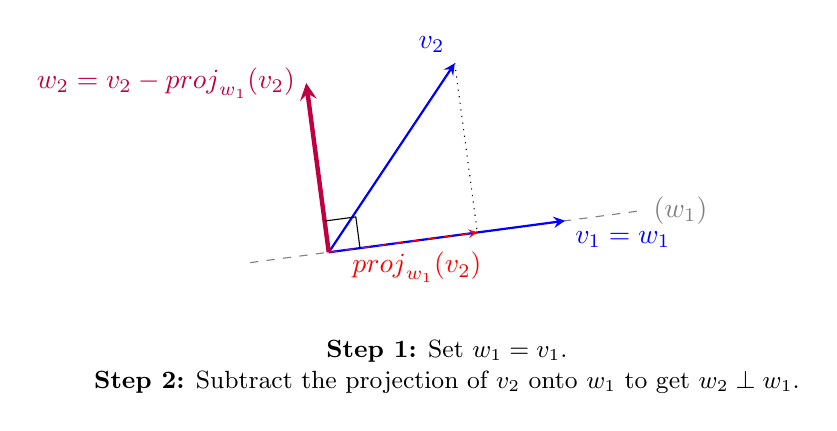
\begin{tikzpicture}[scale=2, >=stealth]
        % Coordinates
        \coordinate (O) at (0,0);
        \coordinate (V1) at (1.5, 0.2);
        \coordinate (V2) at (0.8, 1.2);
        
        % Subspace spanned by w1 (which is v1)
        \draw[dashed, gray] (-0.5, -0.066) -- (2, 0.266) node[right] {$\Sp(w_1)$};
        
        % Original vectors
        \draw[->, thick, blue] (O) -- (V1) node[below right] {$v_1 = w_1$};
        \draw[->, thick, blue] (O) -- (V2) node[above left] {$v_2$};
        
        % Projection of v2 onto w1
        \pgfmathsetmacro{\projcoeff}{((0.8*1.5 + 1.2*0.2)/(1.5*1.5 + 0.2*0.2))}
        \coordinate (Proj) at (\projcoeff*1.5, \projcoeff*0.2);
        \draw[->, dashed, red] (O) -- (Proj) node[pos=0.5, below, xshift=5pt] {$\operatorname{proj}_{w_1}(v_2)$};
        \draw[dotted] (V2) -- (Proj);
        
        % Resulting orthogonal vector w2
        \coordinate (W2) at (0.8-\projcoeff*1.5, 1.2-\projcoeff*0.2);
        \draw[->, ultra thick, purple] (O) -- (W2) node[left] {$w_2 = v_2 - \operatorname{proj}_{w_1}(v_2)$};
        
        % Right angle symbol
        \begin{scope}[rotate={atan2(0.2, 1.5)}]
            \draw (0.2, 0) -- (0.2, 0.2) -- (0, 0.2);
        \end{scope}

        \node[below, align=center, font=\small] at (0.75, -0.5) {
            \textbf{Step 1:} Set $w_1 = v_1$. \\
            \textbf{Step 2:} Subtract the projection of $v_2$ onto $w_1$ to get $w_2 \perp w_1$.
        };
    \end{tikzpicture}
\end{center}

\usetikzlibrary{calc}

\begin{figure}[h]
\centering
\begin{tikzpicture}[scale=1.2]

    % Plane W_{j-1}
    \fill[green!15] (-2,-1) -- (2,-1) -- (3,1) -- (-1,1) -- cycle;
    \draw (-2,-1) -- (2,-1) -- (3,1) -- (-1,1) -- cycle;
    \node at (2.7,-0.9) {$W_{j-1} = \Sp(w_1,\dots,w_{j-1})$};

    % Origin
    \coordinate (O) at (0,0);
    \fill (O) circle (1.2pt);

    % Basis vectors in the plane
    \coordinate (W1) at (1.5,0);
    \coordinate (W2) at (0.8,0.9);
    \coordinate (W3) at (-0.8,0.4);

    \draw[->, thick] (O) -- (W1);
    \node[below] at (W1) {$w_1$};

    \draw[->, thick] (O) -- (W2);
    \node[right] at (W2) {$w_2$};

    \draw[->, thick] (O) -- (W3);
    \node[left] at (W3) {$w_{j-1}$};

    % Projection point (in plane)
    \coordinate (P) at (1.2,0.3);
    \fill (P) circle (1.2pt);
    \node[below right] at (P) {$\Pr_{W_{j-1}}(v_j)$};

    % v_j vector (out of plane)
    \coordinate (V) at (1.6,2.2);
    \draw[->, thick] (O) -- (V);
    \node[right] at (V) {$v_j$};

    % w_j orthogonal component
    \draw[->, thick] (P) -- (V);
    \node[right] at ($(P)!0.5!(V)$) {$w_j$};

    % Projection vector
    \draw[->, thick] (O) -- (P);

    % Orthogonal drop
    \draw[dashed] (V) -- (P);

    % Right angle marker
    \draw ($(P)+(0.15,0)$) -- ($(P)+(0.15,0.15)$) -- ($(P)+(0,0.15)$);

\end{tikzpicture}
\caption{Geometric idea of Gram--Schmidt: the vectors $w_1,\dots,w_{j-1}$ span $W_{j-1}$, 
and $v_j$ decomposes as $v_j = w_j + \Pr_{W_{j-1}}(v_j)$ with $w_j \perp W_{j-1}$.}
\end{figure}

\usetikzlibrary{calc}

\begin{figure}[h]
\centering
\begin{tikzpicture}[scale=1.2]

    % Plane W_{j-1}
    \fill[green!12] (-2,-1) -- (2,-1) -- (3,1) -- (-1,1) -- cycle;
    \draw (-2,-1) -- (2,-1) -- (3,1) -- (-1,1) -- cycle;

    % Light "hand-drawn" strokes
    \foreach \t in {0.2,0.4,0.6,0.8} {
        \draw[green!40, thick] 
            ($(-2,-1)!\t!(-1,1)$) -- ($(2,-1)!\t!(3,1)$);
    }

    % Label of plane
    \node at (-1.8,-1.2) {$W_{j-1}$};

    % Origin
    \coordinate (O) at (0,0);
    \fill (O) circle (1.2pt);

    % Projection point
    \coordinate (P) at (1.1,0.2);
    \fill (P) circle (1.2pt);
    \node[below right] at (P) {$\Pr(v_j)$};

    % v_j vector
    \coordinate (V) at (1.6,2.3);
    \draw[->, thick] (O) -- (V);
    \node[left] at ($(O)!0.7!(V)$) {$v_j$};

    % w_j vector
    \draw[->, thick] (P) -- (V);
    \node[right] at ($(P)!0.5!(V)$) {$w_j$};

    % projection vector
    \draw[->, thick] (O) -- (P);

    % dashed orthogonal drop
    \draw[dashed] (V) -- (P);

    % right angle marker
    \draw ($(P)+(0.12,0)$) -- ($(P)+(0.12,0.12)$) -- ($(P)+(0,0.12)$);

    % Span text
    \node at (2.8,0.6) 
    {$\Sp(v_1,\dots,v_{j-1})=\Sp(w_1,\dots,w_{j-1})=W_{j-1}$};

    % Formulas (like in sketch)
    \node at (3.2,2.0) 
    {$w_j = v_j - \Pr_{W_{j-1}}(v_j)$};

    \node at (3.2,1.4) 
    {$v_j = w_j + \Pr_{W_{j-1}}(v_j)$};

\end{tikzpicture}
\caption{Geometric idea behind the Gram--Schmidt process.}
\end{figure}


\begin{remark}
    In practice, the Gram-Schmidt process is often followed by a normalization step to produce an orthonormal basis. This two-stage process is essential for many numerical algorithms and theoretical results in linear algebra, such as the $QR$ decomposition.
\end{remark}